\documentclass[tikz,border=8pt]{standalone}
% Shared look for every TikZ diagram. Load with % Shared look for every TikZ diagram. Load with % Shared look for every TikZ diagram. Load with \input{../../tools/tikz-style.tex}
\usepackage[T1]{fontenc}
\usepackage{lmodern}
\renewcommand{\sfdefault}{lmr}  % diagrams use the same serif as the text
\usetikzlibrary{arrows.meta, positioning, shapes.geometric, calc, fit, backgrounds}
\definecolor{cblue}{HTML}{4C78A8}
\definecolor{corange}{HTML}{F58518}
\definecolor{cgreen}{HTML}{54A24B}
\definecolor{cred}{HTML}{E45756}
\definecolor{cpurple}{HTML}{B279A2}
\definecolor{cgrey}{HTML}{6B6B6B}
\tikzset{
  every picture/.style={font=\sffamily, line width=1.2pt},
  box/.style={draw=#1, fill=#1!12, rounded corners=4pt, align=center, inner sep=7pt, minimum height=1.1cm},
  box/.default=cgrey,
  arrow/.style={-{Stealth[length=3mm]}, draw=cgrey, line width=1.4pt},
  title/.style={font=\sffamily\bfseries\Large},
  note/.style={font=\sffamily\small, text=cgrey, align=center},
}
\AtBeginDocument{\hyphenpenalty=10000 \exhyphenpenalty=10000}

\usepackage[T1]{fontenc}
\usepackage{lmodern}
\renewcommand{\sfdefault}{lmr}  % diagrams use the same serif as the text
\usetikzlibrary{arrows.meta, positioning, shapes.geometric, calc, fit, backgrounds}
\definecolor{cblue}{HTML}{4C78A8}
\definecolor{corange}{HTML}{F58518}
\definecolor{cgreen}{HTML}{54A24B}
\definecolor{cred}{HTML}{E45756}
\definecolor{cpurple}{HTML}{B279A2}
\definecolor{cgrey}{HTML}{6B6B6B}
\tikzset{
  every picture/.style={font=\sffamily, line width=1.2pt},
  box/.style={draw=#1, fill=#1!12, rounded corners=4pt, align=center, inner sep=7pt, minimum height=1.1cm},
  box/.default=cgrey,
  arrow/.style={-{Stealth[length=3mm]}, draw=cgrey, line width=1.4pt},
  title/.style={font=\sffamily\bfseries\Large},
  note/.style={font=\sffamily\small, text=cgrey, align=center},
}
\AtBeginDocument{\hyphenpenalty=10000 \exhyphenpenalty=10000}

\usepackage[T1]{fontenc}
\usepackage{lmodern}
\renewcommand{\sfdefault}{lmr}  % diagrams use the same serif as the text
\usetikzlibrary{arrows.meta, positioning, shapes.geometric, calc, fit, backgrounds}
\definecolor{cblue}{HTML}{4C78A8}
\definecolor{corange}{HTML}{F58518}
\definecolor{cgreen}{HTML}{54A24B}
\definecolor{cred}{HTML}{E45756}
\definecolor{cpurple}{HTML}{B279A2}
\definecolor{cgrey}{HTML}{6B6B6B}
\tikzset{
  every picture/.style={font=\sffamily, line width=1.2pt},
  box/.style={draw=#1, fill=#1!12, rounded corners=4pt, align=center, inner sep=7pt, minimum height=1.1cm},
  box/.default=cgrey,
  arrow/.style={-{Stealth[length=3mm]}, draw=cgrey, line width=1.4pt},
  title/.style={font=\sffamily\bfseries\Large},
  note/.style={font=\sffamily\small, text=cgrey, align=center},
}
\AtBeginDocument{\hyphenpenalty=10000 \exhyphenpenalty=10000}

\begin{document}
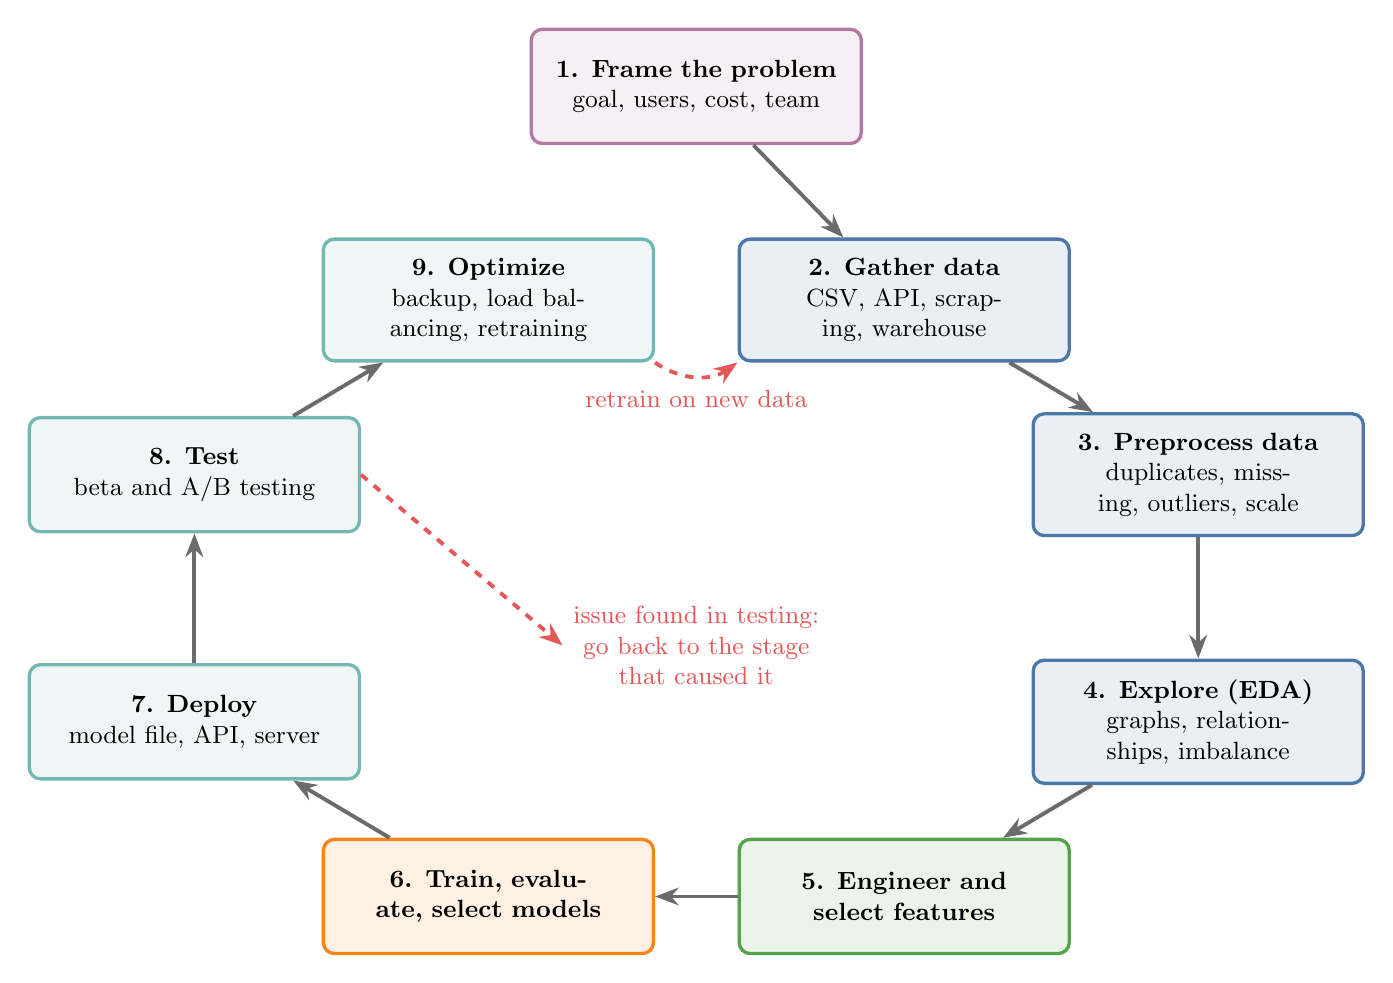
\begin{tikzpicture}
  \definecolor{cteal}{HTML}{72B7B2}
  \tikzset{st/.style={box=#1, minimum width=3.9cm, text width=3.7cm, minimum height=1.45cm, font=\small}}
  % Stage 1 happens first; stages 2-9 form the cycle on an ellipse
  \node[st=cpurple] (s1) at (0,6.5) {\textbf{1. Frame the problem}\\goal, users, cost, team};
  \foreach \i/\a/\t/\c in {
      2/67.5/{\textbf{2. Gather data}\\CSV, API, scraping, warehouse}/cblue,
      3/22.5/{\textbf{3. Preprocess data}\\duplicates, missing, outliers, scale}/cblue,
      4/-22.5/{\textbf{4. Explore (EDA)}\\graphs, relationships, imbalance}/cblue,
      5/-67.5/{\textbf{5. Engineer and select features}}/cgreen,
      6/-112.5/{\textbf{6. Train, evaluate, select models}}/corange,
      7/-157.5/{\textbf{7. Deploy}\\model file, API, server}/cteal,
      8/157.5/{\textbf{8. Test}\\beta and A/B testing}/cteal,
      9/112.5/{\textbf{9. Optimize}\\backup, load balancing, retraining}/cteal}
    \node[st=\c] (s\i) at ({6.9*cos(\a)},{4.1*sin(\a)}) {\t};
  \draw[arrow] (s1) -- (s2);
  \foreach \a/\b in {2/3, 3/4, 4/5, 5/6, 6/7, 7/8, 8/9} \draw[arrow] (s\a) -- (s\b);
  % Loops back
  \draw[arrow, draw=cred, dashed] (s9.south east) to[bend right=35] node[font=\small, text=cred, below=1pt] {retrain on new data} (s2.south west);
  \node[font=\small, text=cred, align=center] (fix) at (0,-0.6) {issue found in testing:\\go back to the stage\\that caused it};
  \draw[arrow, draw=cred, dashed] (s8.east) -- (fix.west);
\end{tikzpicture}
\end{document}
